\section{Cálculos teóricos}

Para empezar a operar el sistema LTI estocástico, es necesario hacer algunos cálculos iniciales, como correlaciones varias.

Como $h(n)$ es la respuesta impulsiva a un filtro FIR de largo $L$, la misma será una secuencia lineal del siguiente tipo:
$h(n) = \{h_0, h_1, \cdots, h_{L-1}\}$. Análogamente, el ecualizador descripto por $w(n)$ también se desarrollará como una secuencia
de largo $M$: $w(n) = \{w_0, w_1, \cdots, w_{M-1}\}$. Por tanto, ambas respuestas son nulas a valores de $n$ negativos (causales) y
superiores a su largo.

Se sabe que $X(n)\in\{-1,1\}$ y, para cada instante distinto, las variables aleatorias son independientes e idénticamente distribuidas,
por lo que tendrán media nula constante. Asumiendo que es un proceso estacionario en sentido amplio, es posible calcular su función de
autocorrelación de la siguiente manera
\begin{align*}
    R_X(k) &= \mathbb{E}[X(n)X(n+k)] =
    \begin{cases}
        \mathbb{E}[\underbrace{X^2(n)}_{ = 1}] & k = 0 \\
        \underbrace{\mathbb{E}[X(n)]\mathbb{E}[X(n+k)]}_{=0} & k \neq 0
    \end{cases}\\
    &= \delta(k).
\end{align*}

Al proceso de salida del filtro FIR se le suma un ruido blanco $V(n)$ de varianza $\sigma^2$ y media nula independiente a $X(n)$,
definiéndose \[Y(n) = (h * X)(n) + V(n) = \sum_{i=1}^{L-1} h(i)X(n - i) + V(n)\] por lo que es posible calcular su función de
autocorrelación de la siguiente manera.

\begin{align*}
    R_Y(k) &= \mathbb{E}[Y(n)Y(n+k)]\\
    &= \mathbb{E}\left[\left(\sum_{i=1}^{L-1} h(i)X(n - i) + V(n)\right)\left(\sum_{j=1}^{L-1} h(j) X(n + k - j) + V(n+k)\right)\right]\\
    &= \sum_{i=1}^{L-1}\sum_{j=1}^{L-1} h(i)h(j) \mathbb{E}[X(n - i)X(n + k - j)] + \mathbb{E}[V(n)V(n + k)]\\
    &= \sum_{i=1}^{L-1}\sum_{j=1}^{L-1} h(i)h(j) R_X(k+i-j) + R_V(k) = \sum_{i=1}^{L-1}\sum_{j=1}^{L-1} h(i)h(j) \delta(k+i-j) + \sigma_V^2\delta(k)\\
    &= \sum_{i=1}^{L-1} h(i)h(k+i) + \sigma_V^2\delta(k) = \sum_{n = 1 - L}^{-1} h(-n)h(k-n) + \sigma_V^2\delta(k) \underset{\substack{\downarrow \\ \tilde{h}(n) = h(-n)}}{=} (\tilde{h}*h)(k) + \sigma_V^2\delta(k)\\
\end{align*}

Se procede a continuación con el cálculo de la correlación cruzada entre $X(n)$ e $Y(n)$.
\begin{align*}
    R_{XY}(k) &= \mathbb{E}[X(n)Y(n+k)] = \mathbb{E}\left[X(n)\left(\sum_{j=1}^{L-1} h(j)X(n + k - j) + V(n+k)\right)\right]\\
    &= \sum_{j=1}^{L-1} h(j) R_X(k-j) = \sum_{j=1}^{L-1} h(j) \delta(k-j) = h(k)
\end{align*}

Los resultados obtenidos son los siguientes:
\begin{align*}
    \boxed{R_X(k) = \delta(k)} &&
    \boxed{R_Y(k) = (\tilde{h} * h)(k) + \sigma_V^2 \delta(k)} &&
    \boxed{R_{XY}(k) = h(k)}
\end{align*}

\section{Elección óptima del filtro ecualizador}
\label{sec:eleccion-optima}

La solución óptima para los coeficientes del ecualizador debe cumplir con la siguiente expresión:
\begin{equation*}
	\mathbf{R}_Y \mathbf{w}_o = \mathbf{R}_{YX},
\end{equation*}
donde $\mathbf{R}_Y$ es la matriz de Toeplitz de la autocorrelación de $Y$. Luego, la matriz $\mathbf{R}_{YX}$ es:
\[
\mathbf{R}_{YX} = \mathbb{E}
\begin{bmatrix}
	y(n) x(n) \\
	y(n-1) x(n) \\
	\vdots \\
	y(n - M + 1) x(n)
\end{bmatrix}
=
\begin{bmatrix}
	R_{YX}(0) \\
	R_{YX}(1) \\
	\vdots \\
	R_{YX}(M-1)
\end{bmatrix}
=
\begin{bmatrix}
	h(0) \\
	h(-1) \\
	\vdots \\
	h(-M+1)
\end{bmatrix}
=
\begin{bmatrix}
	h(0) \\
	0 \\
	\vdots \\
	0
\end{bmatrix}
\]

Finalmente $\mathbf{w}_o$ es un vector que se obtiene de operar de la siguiente manera con las matrices previamente mencionadas.

\begin{equation}
	\mathbf{w}_o = \mathbf{R}_Y^{-1} \cdot \mathbf{R}_{YX}
\end{equation}

\section{Simulación del sistema}

Como se demuestra en la Sección~\ref{sec:eleccion-optima}, las matrices con las que se calculan los coeficientes óptimos para el ecualizador dependen solamente de los coeficientes del modelo del canal. Luego se simuló la secuencia $X(n)$ y en base a ella se calcularon las secuencias $Y(n)$ y $Z(n)$ usando la funcion \verb*|filter| con $\mathbf{h}$ y $\mathbf{w}_o$. La figura~\ref{fig:ej3_x} muestra como la autocorrelación de $X(n)$ resulta en algo similar a una delta en el origen y la PSD resulta ruidosa, pero relativamente constante.

\begin{figure}[!hbp]
	\centering
    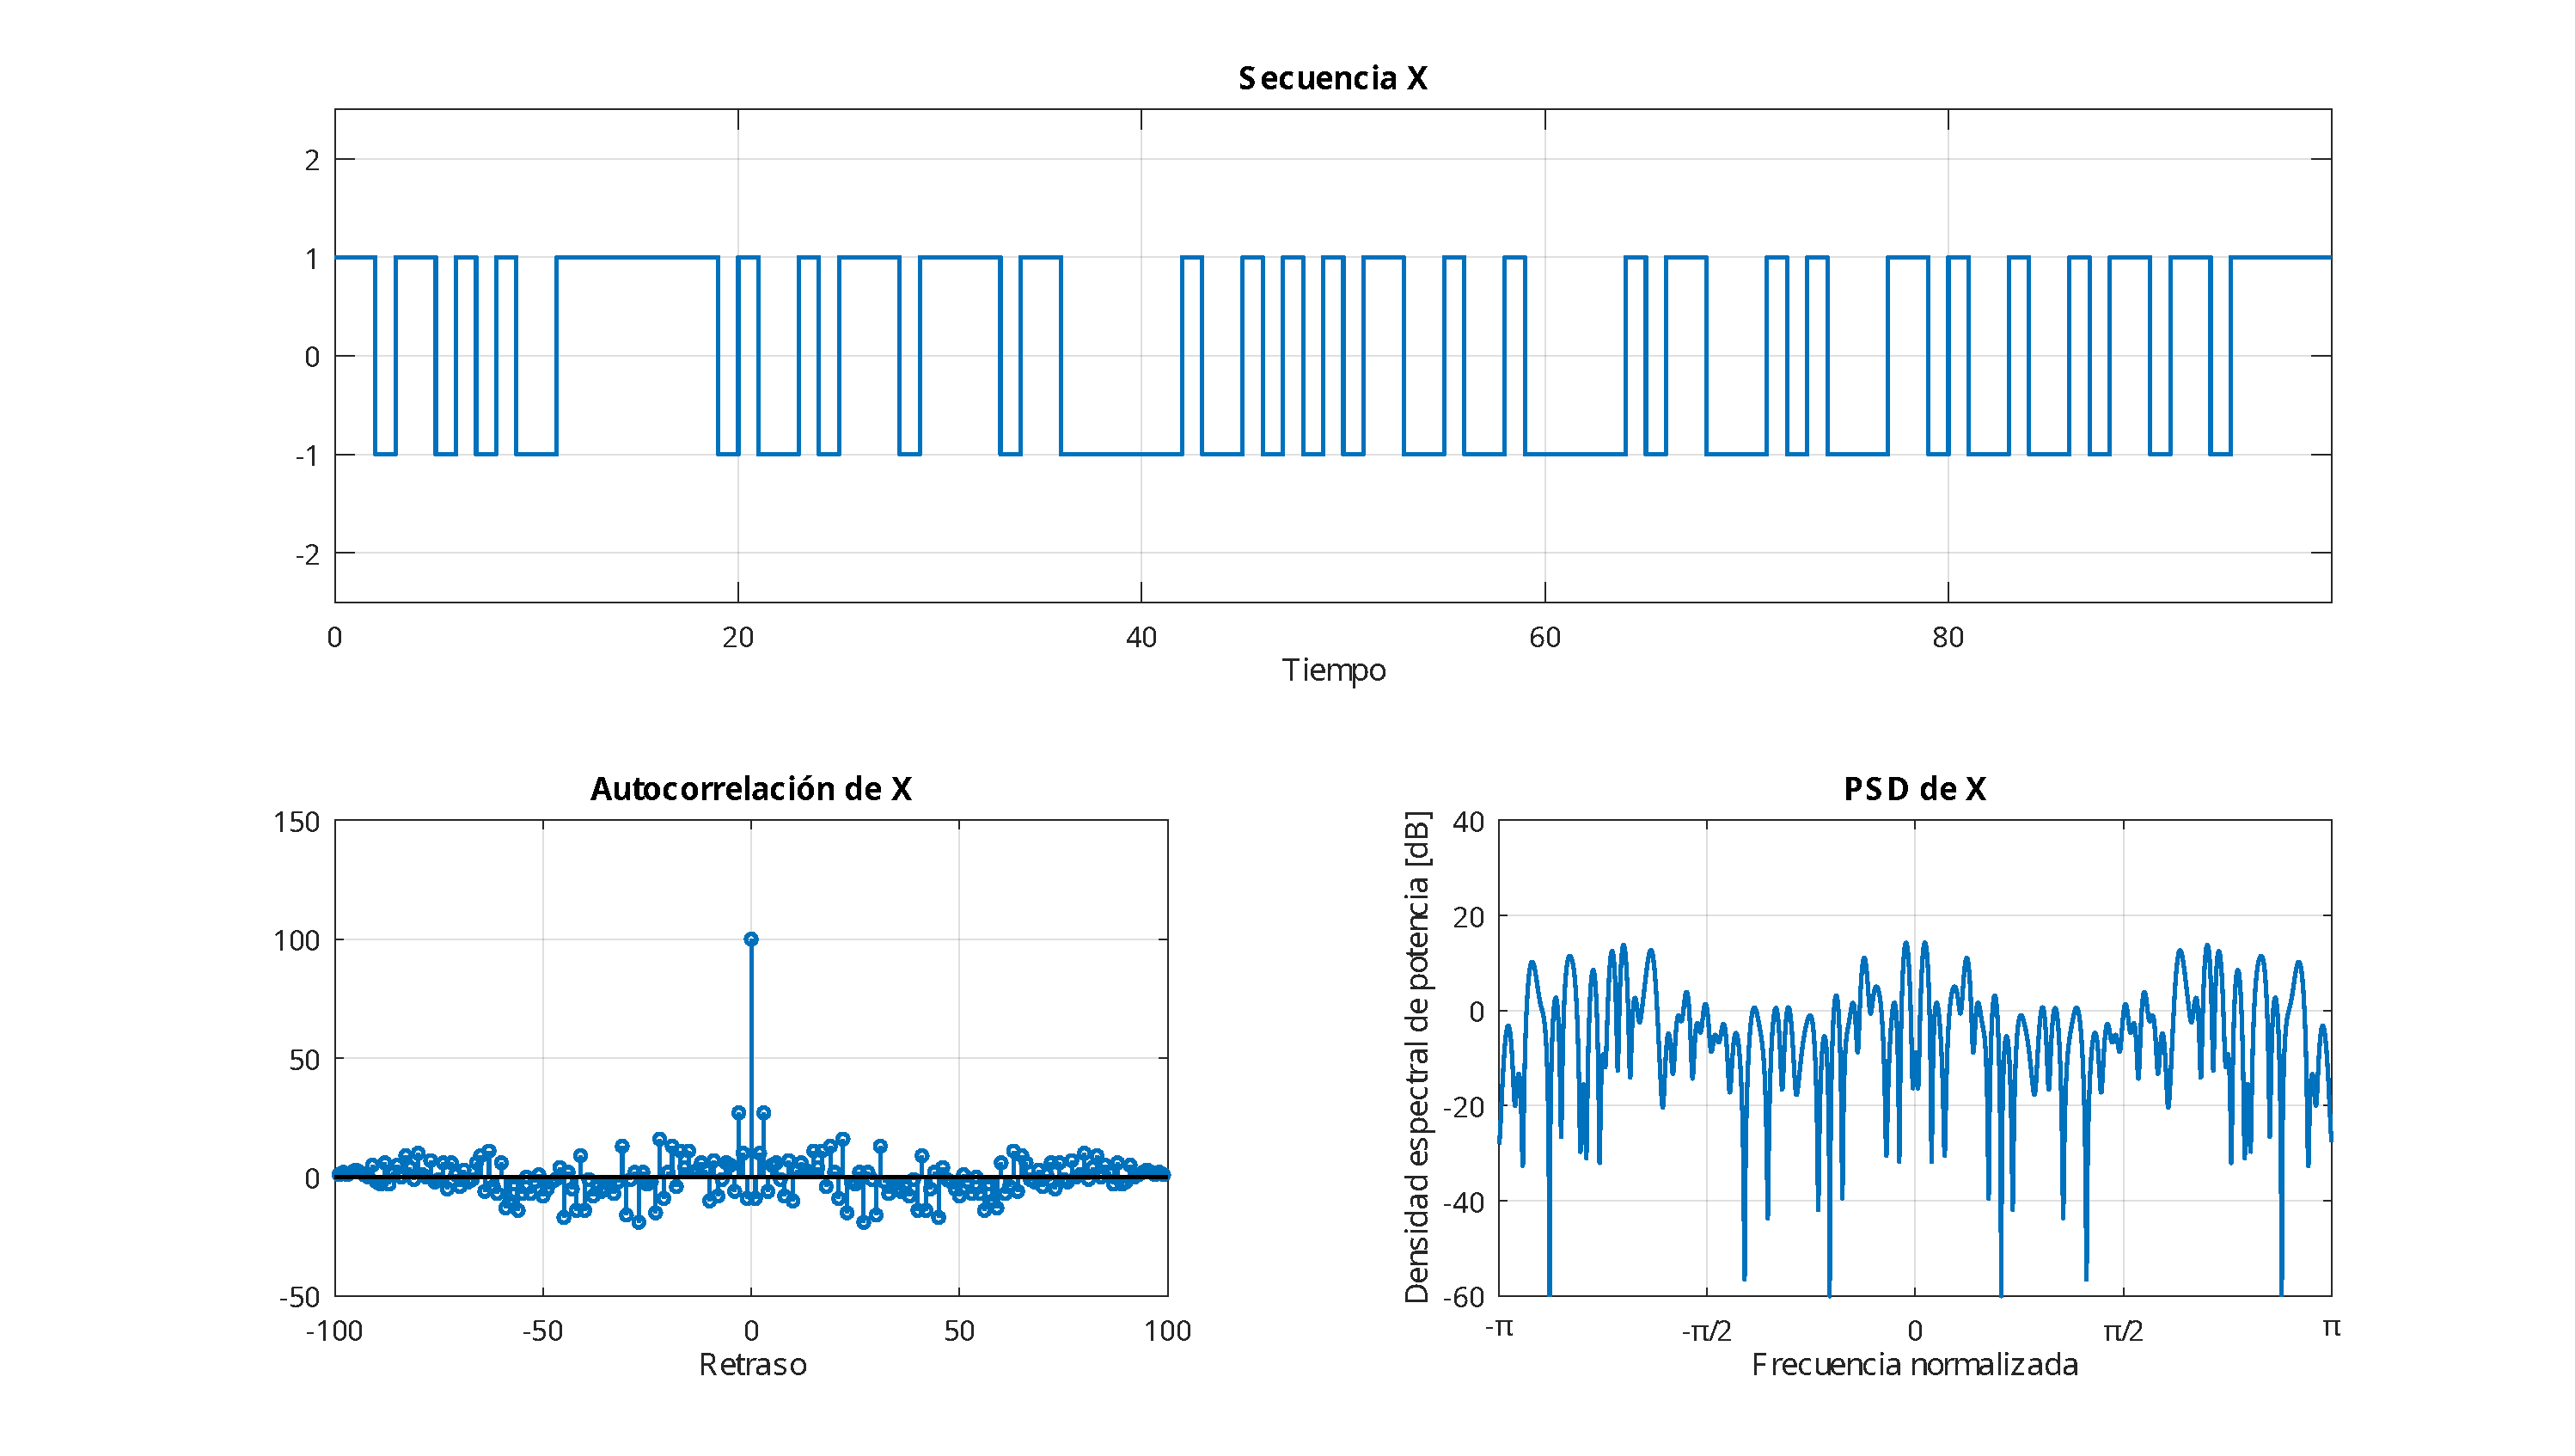
\includegraphics[width=1\linewidth,trim=4cm 0 4cm 0,clip]{img/ej3_x.pdf}
	\caption{Secuencia, autocorrelación y PSD de $X(n)$.}
	\label{fig:ej3_x}
\end{figure}

En la figura~\ref{fig:ej3_y} se observan los atributos de la secuencia $Y(n)$, es decir cómo termina $X(n)$ una vez que atraviesa el canal. Como era de esperar, la señal se distorsiona considerablemente, ya que tanto la secuencia, como su autocorrelación y PSD difieren mucho de $X(n)$.

\begin{figure}[!hbp]
	\centering
	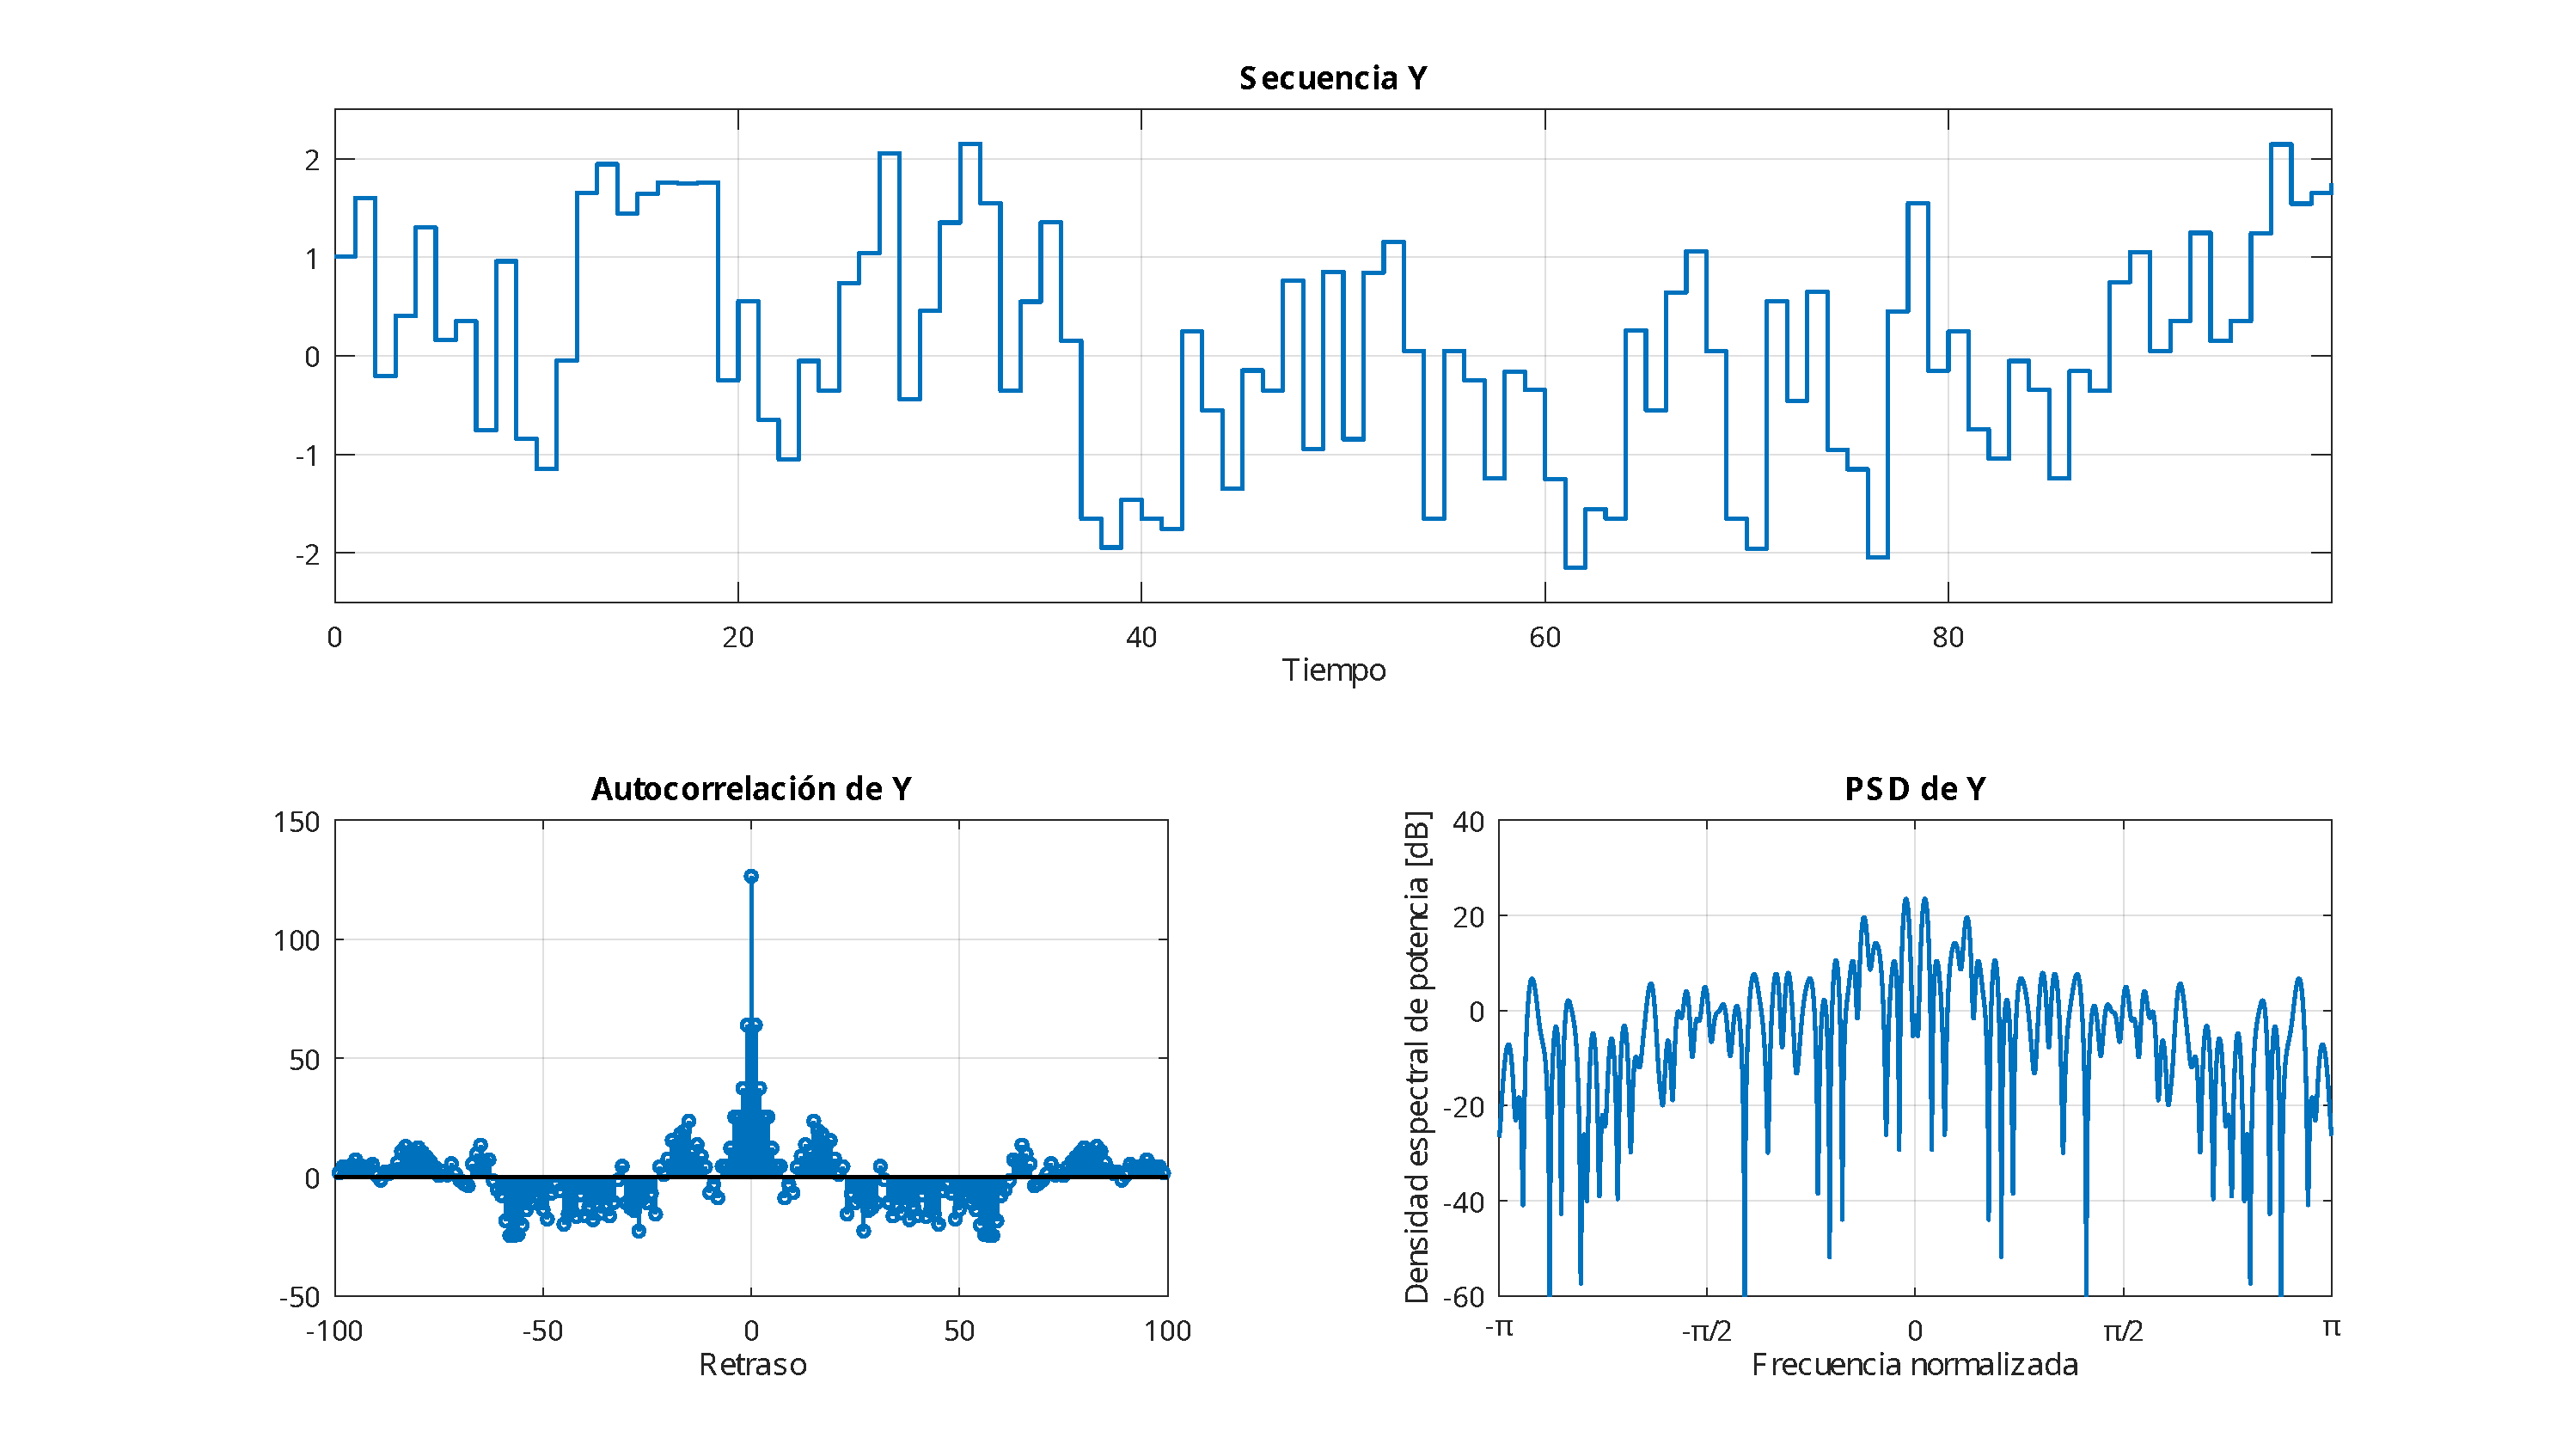
\includegraphics[width=1\linewidth,trim=4cm 0 4cm 0,clip]{img/ej3_y.pdf}
	\caption{Secuencia, autocorrelación y PSD de $Y(n)$.}
	\label{fig:ej3_y}
\end{figure}

Por último, la figura~\ref{fig:ej3_z} muestra una secuencia casi idéntica a la de entrada, demostrando que el ecualizador funcionó correctamente.

\begin{figure}[!hbp]
	\centering
	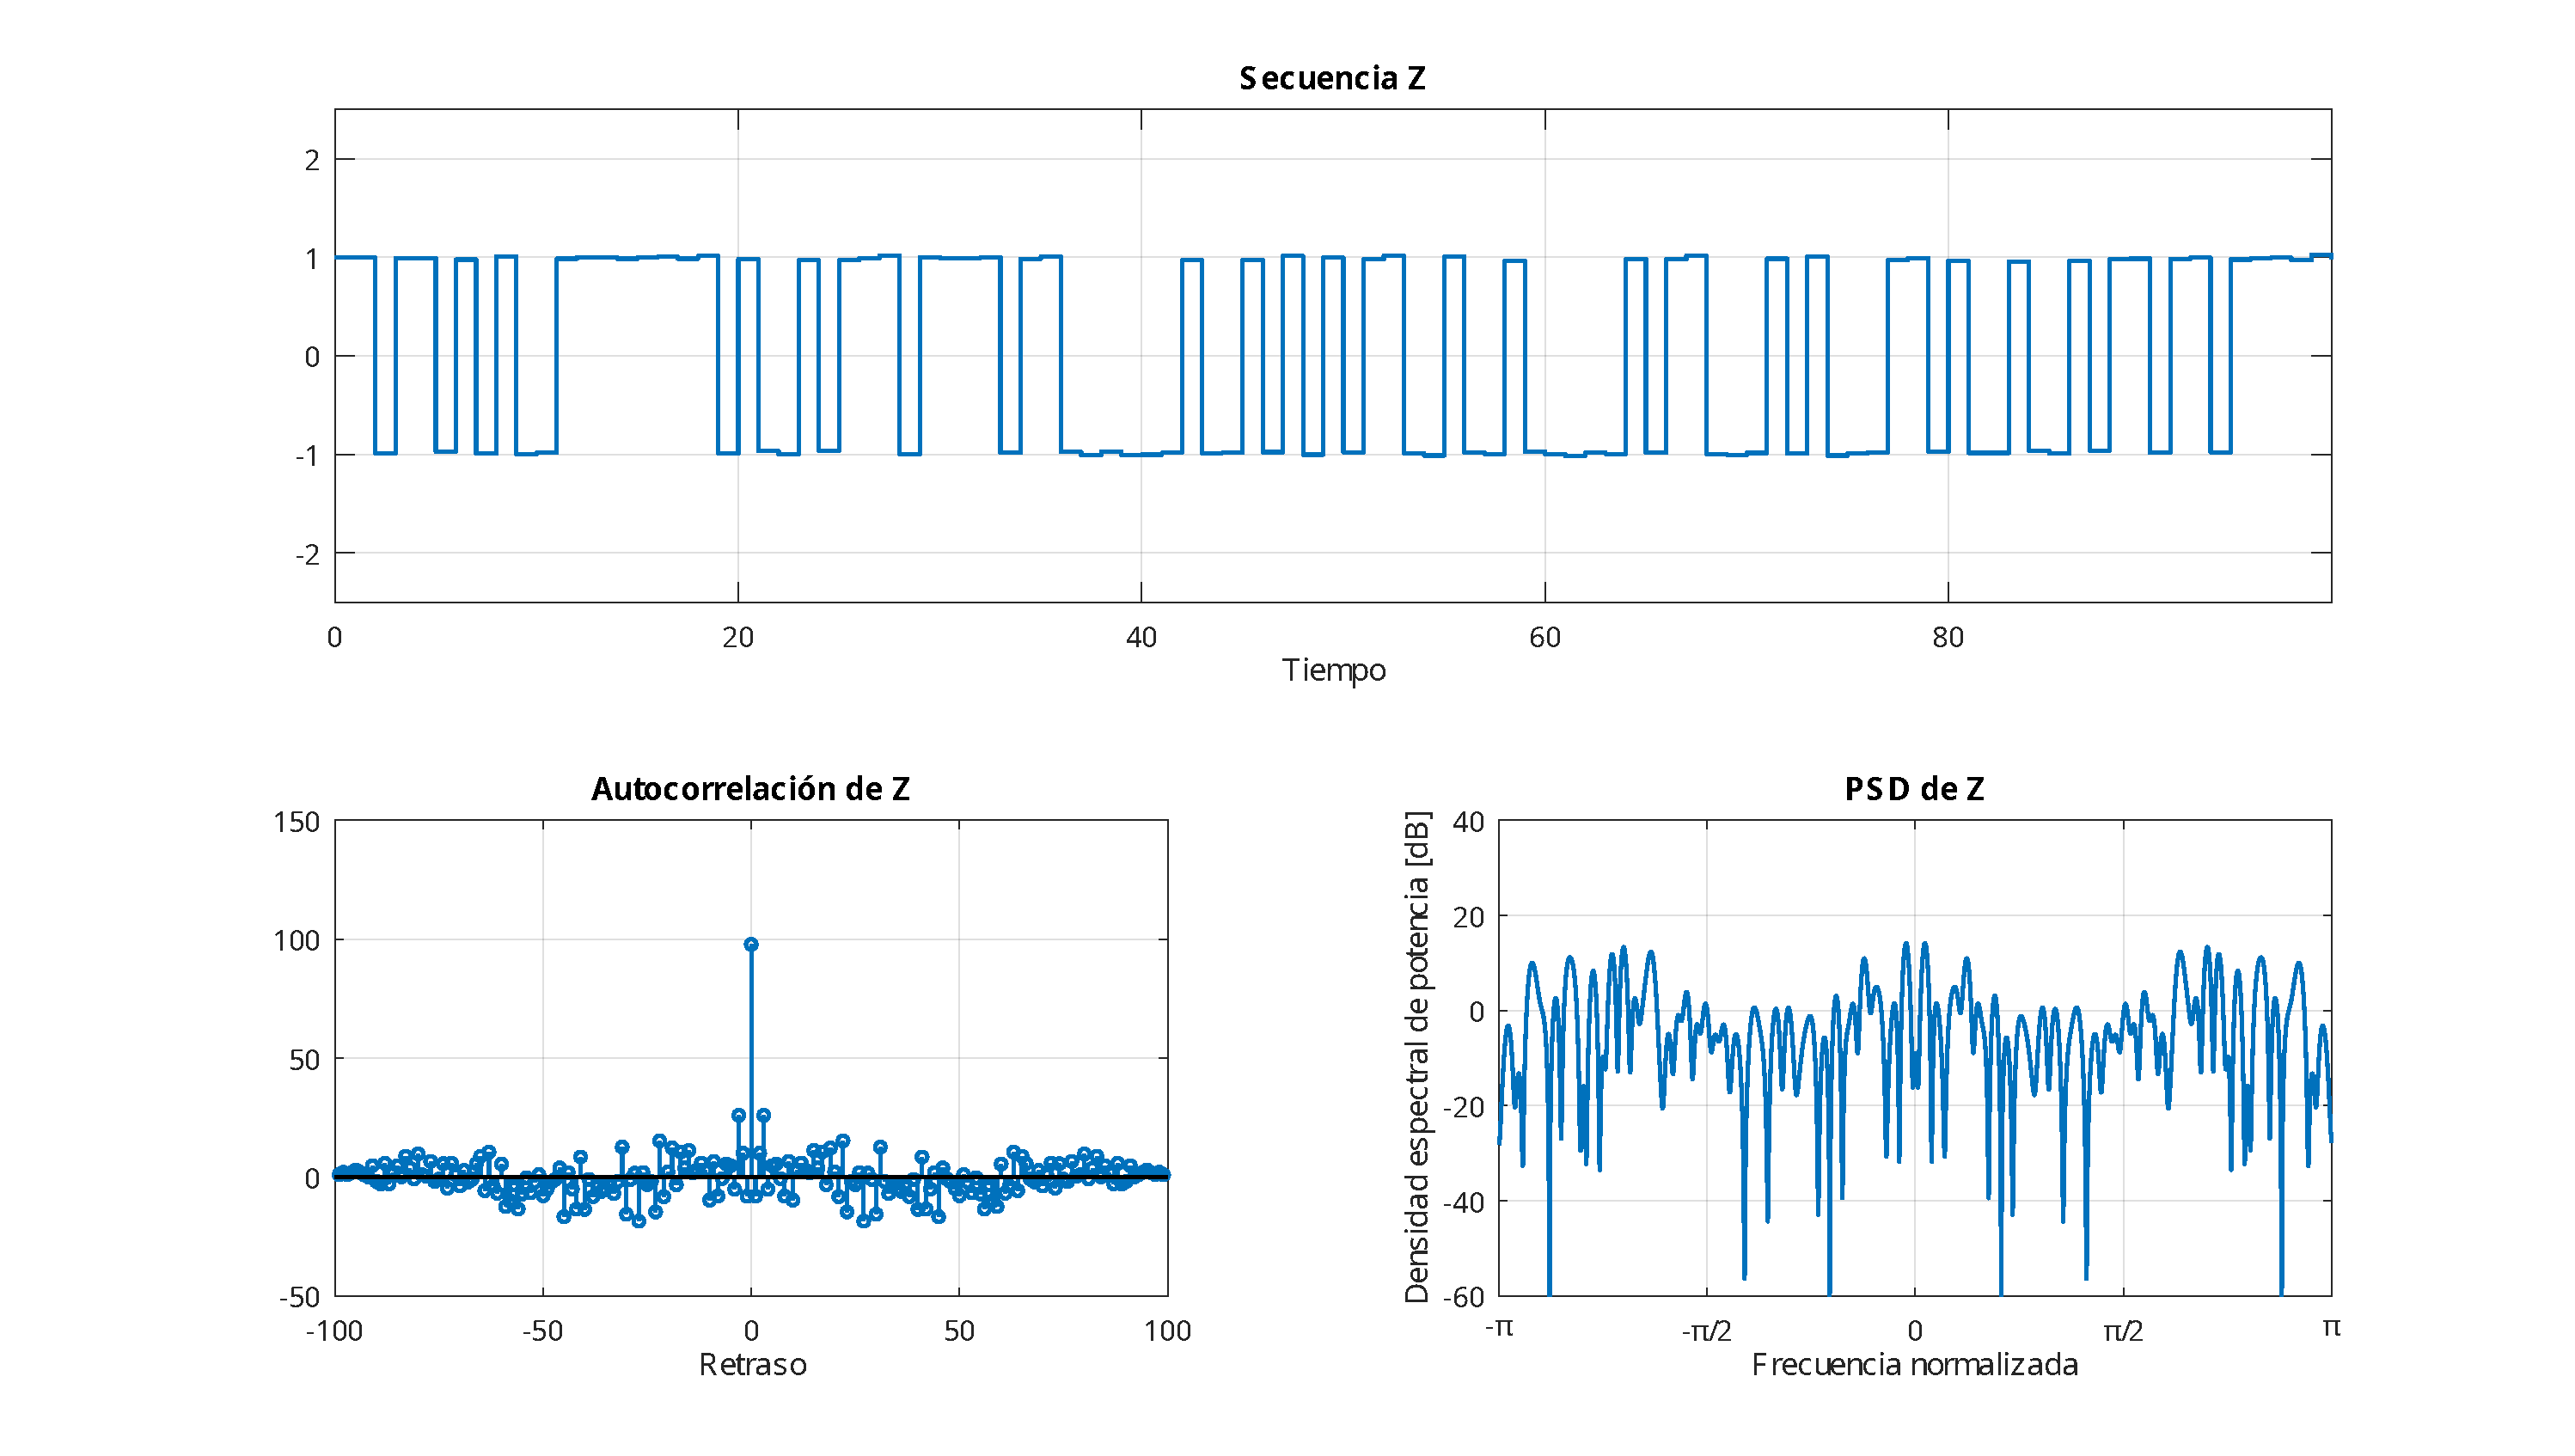
\includegraphics[width=1\linewidth,trim=4cm 0 4cm 0,clip]{img/ej3_z.pdf}
	\caption{Secuencia, autocorrelación y PSD de $Z(n)$.}
	\label{fig:ej3_z}
\end{figure}

En la figura~\ref{fig:ej3_coef} se muestra una comparación de los coeficientes del modelo del canal y los coeficientes del ecualizador obtenidos.

\begin{figure}[!hbp]
	\centering
	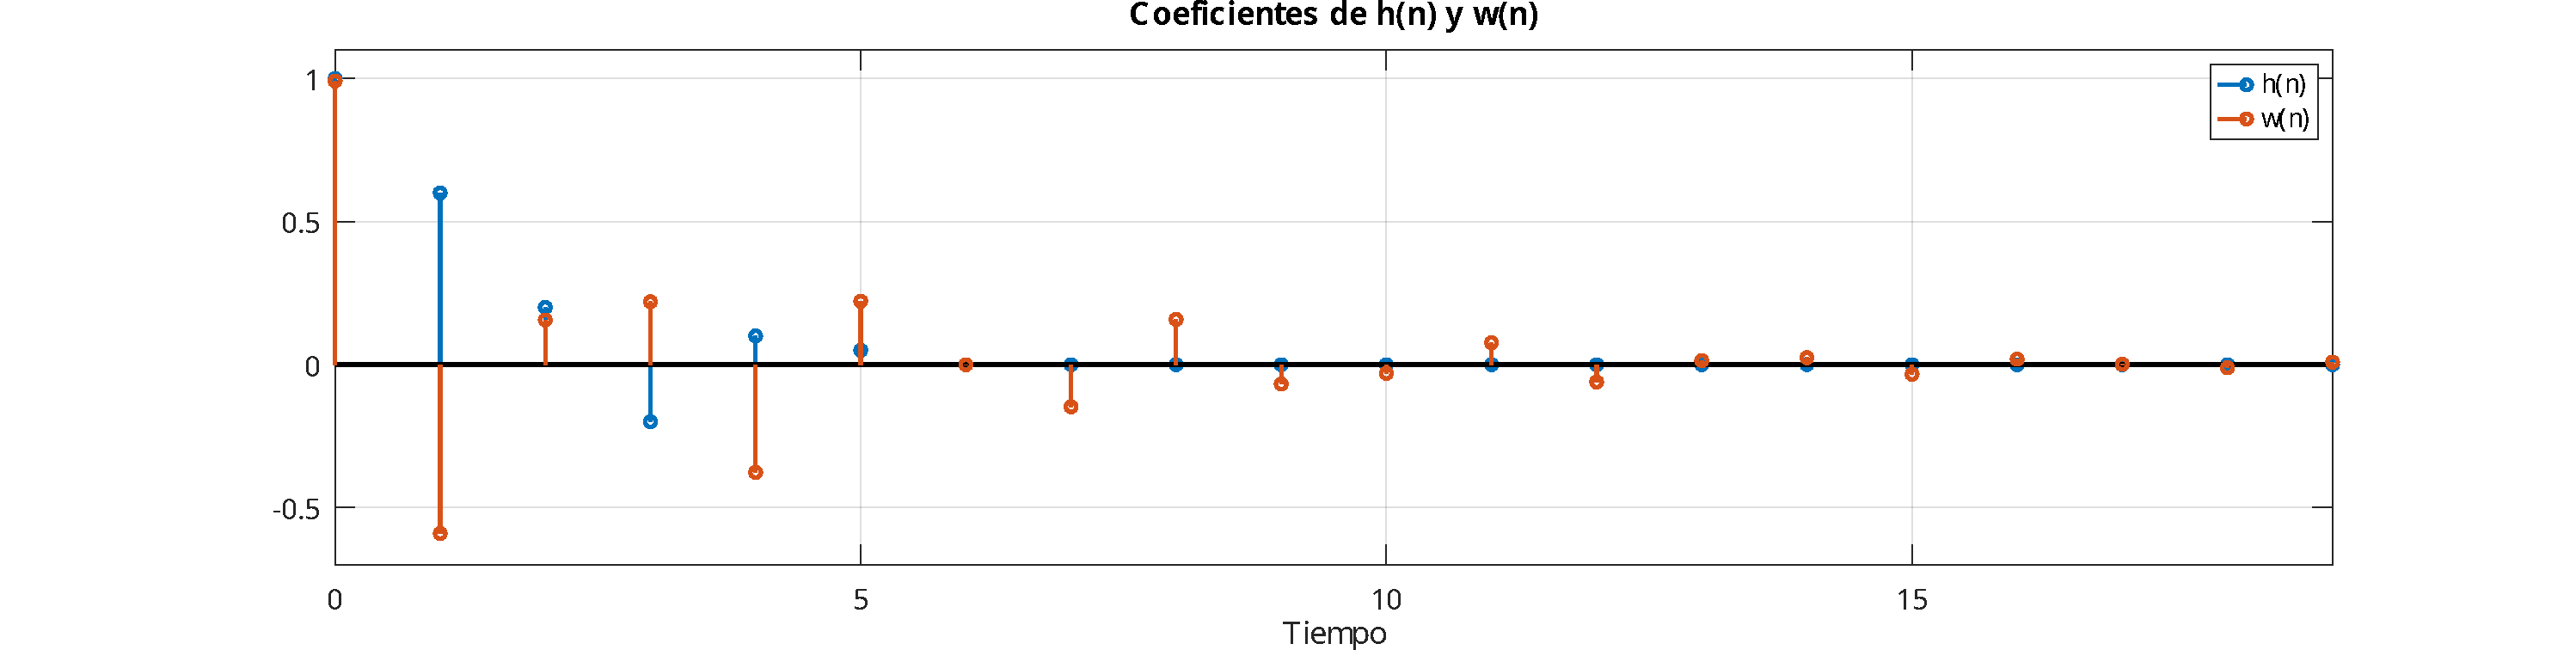
\includegraphics[width=1\linewidth,trim=4cm 0 4cm 0,clip]{img/ej3_coef.pdf}
	\caption{Comparación de $h$ y $w$.}
	\label{fig:ej3_coef}
\end{figure}

\clearpage

\section{Ejercicio 4}

En esta instancia se analiza como la longitud del filtro ecualizador afecta la calidad de la señal de salida.
